\documentclass[a4paper,12pt,dutch]{article}
\usepackage{glossaries}
\usepackage[T1]{fontenc}
\usepackage{babel}
\usepackage{graphicx}
\usepackage[table,xcdraw]{xcolor}
\usepackage{hyperref}
\usepackage{blindtext}
\usepackage{geometry}
\usepackage{parskip}
\usepackage{mathtools}
\usepackage{siunitx}
\usepackage{listings}
\usepackage{csquotes}
\usepackage{caption}
\usepackage{subcaption}
\usepackage{comment}

% %% Some packages you will need
% \usepackage{pgfplots}
% \usepackage{pgfplotstable}
% \usepackage{booktabs}
% \usepackage{array}
% \usepackage{colortbl}


\definecolor{arduinoorange}{HTML}{FFA500}
\definecolor{arduinogray}{HTML}{808080}
\definecolor{arduinoblue}{HTML}{007ACC}
\definecolor{arduinogreen}{HTML}{469B00}

\lstset{
  language=C++,
  basicstyle=\ttfamily\footnotesize,
  keywordstyle=\color{arduinoorange},
  stringstyle=\color{arduinogreen},
  commentstyle=\color{arduinogray},
  moredelim=[s][\color{arduinoblue}]{\#}{\ },
  morekeywords={digitalRead,digitalWrite,pinMode,analogRead,analogWrite,Serial,begin,HIGH,LOW},
  frame=tb,
  tabsize=4,
  showstringspaces=false,
  breaklines=true,
  numbers=left,
  numberstyle=\tiny\color{arduinogray},
  numbersep=5pt,
  extendedchars=true,
  literate={á}{{\'a}}1 {ã}{{\~a}}1 {é}{{\'e}}1,
}

\lstdefinestyle{Arduino}
{
  language=C++,
  basicstyle=\ttfamily\footnotesize,
  keywordstyle=\color{arduinoorange},
  stringstyle=\color{arduinogreen},
  commentstyle=\color{arduinogray},
  moredelim=[s][\color{arduinoblue}]{\#}{\ },
  morekeywords={digitalRead,digitalWrite,pinMode,analogRead,analogWrite,Serial,begin},
  frame=tb,
  tabsize=4,
  showstringspaces=false,
  breaklines=true,
  numbers=left,
  numberstyle=\tiny\color{arduinogray},
  numbersep=5pt,
  extendedchars=true,
  literate={á}{{\'a}}1 {ã}{{\~a}}1 {é}{{\'e}}1,
  backgroundcolor=\color{black!85},
  rulecolor=\color{arduinoorange},
  frame=single,
  frameround=tttt,
  framexleftmargin=6pt,
  framexrightmargin=6pt,
  framextopmargin=6pt,
  framexbottommargin=6pt,
  breaklines=true,
  postbreak=\raisebox{0ex}[0ex][0ex]{\ensuremath{\color{red}\hookrightarrow\space}},
}

\usepackage[
    backend=biber,
    backref=true,
    backrefstyle=none,
    sortcites=true,
    sorting=none,
    doi=false, % doi informatie wordt niet weergegeven
    %uniquename=true,
    %uniquelist=true,
    maxcitenames=3,
    %issn=false, werkt niet
    language=american
]{biblatex}
\addbibresource{information/Bronnen.bib}
\DefineBibliographyStrings{dutch}{
    backrefpage = {blz.},
    backrefpages = {blz.},
}
\makeglossaries
\definecolor{Grey1}{HTML}{343434}
\graphicspath{{./Media/Figuren/}}
 \geometry{
 a4paper,
 total={170mm,257mm},
 left=20mm,
 top=20mm,
 }
\hypersetup{
    colorlinks=true,
    linkcolor=blue,
    filecolor=magenta,      
    urlcolor=cyan,
    pdftitle={Overleaf Example},
    pdfpagemode=FullScreen,
    }


\begin{document}
\title{

\includegraphics[width=3.5in]{IMG/HHS.png} \\
\vspace*{2in}
\textbf{Project 3}\\
\textit{PVA Duurzame Energie}\\
Versie 1
}
\author{
\vspace*{2.5in} \\
  Geschreven door:\\
  Laurens van der Drift\\
  Tommy Dobos\\
		\vspace*{0.2in} \\
		De Haagse Hogeschool\\
        \textbf{Elektrotechniek}\\
        Delft, Nederland
       } 
\maketitle
\phantomsection
\section*{Versie Historie} \addcontentsline{toc}{section}{Versie Historie}

\begin{table}[h]
\begin{tabular}{|l|l|l|l|}
\hline
\rowcolor[HTML]{4472C4} 
{\color[HTML]{FFFFFF} \textbf{Versie}} &
  {\color[HTML]{FFFFFF} \textbf{Datum}} &
  {\color[HTML]{FFFFFF} \textbf{Wijzigingen}} &
  {\color[HTML]{FFFFFF} \textbf{Auteur}} \\ \hline
\rowcolor[HTML]{D9E1F2} 
1.0 &
  \multicolumn{1}{c|}{\cellcolor[HTML]{D9E1F2}30-08-2023} &
 N.v.t. &
  Cleaneco \\ \hline

% \rowcolor[HTML]{FFFFFF} 
% 2.0 &
%   \multicolumn{1}{c|}{\cellcolor[HTML]{FFFFFF}7-4-2023} &
%  Feedback van FeedbackFruits toegepast &
%   Infra   Vroom \\ \hline

% \rowcolor[HTML]{D9E1F2} 
% 3.0 &
%   \multicolumn{1}{c|}{\cellcolor[HTML]{D9E1F2}4-6-2023} &
%  Bijgewerkt voor Assessment 3 &
%   Infra   Vroom \\ \hline

\end{tabular}
\end{table}
%\addcontentsline{toc}{section}{Verklarende Woordenlijst}
\printglossaries
\newglossaryentry{tender}
{
    name=\textit{tender},
    description={De inschrijving om op een kavel een wind turbine park te bouwen.}
}
\newglossaryentry{energie akkoord}
{
    name=\textit{energie akkoord},
    description={Het Energieakkoord vertegenwoordigt duurzame groei, met betrokkenheid van 40+ organisaties waaronder overheid, werkgevers en milieuactivisten. Het bevat afspraken over energiebesparing, schonere technologie en klimaatbeleid.}
}

\newpage
\tableofcontents
\section{Achtergrond}
Cleaneco is een bedrijf ontstaan in augustes 2023 te Delft en is opgericht door Laurens van der Drift en Tommy Dobos.

Ingenieurs- en consultancybureau Worley heeft het ontwerp bedrijf Cleaneco aangenomen om een \gls{offshore} windpark te ontwerpen op kavel VI en VII van Hollandse Kust West en hiervoor de \gls{tender} te schrijven voor Rijkswaterstaat. 

De reden voor de aanleg van het windturbinepark op zee is het \gls{energie akkoord}\cite{energieakkoord} van 2013. In dit akkoord is afgesproken dat in 2023, 4.450MW aan windvermogen op zee opgewekt moet worden. Met als doel genoeg vermogen opwekken voor vijf miljoen huishoudens. 

\section{De projectopdracht}
\subsection{Project naam}
Voor dit project, Project Windpark Op Zee is het bedrijf Cleaneco in dienst genomen door Worley. 

\subsection{Probleem}
De Nederlandse overheid moet voldoen aan het \gls{energie akkoord}, dat is vastgelegd op 6 september 2013. Dit akkoord stelt dat tegen 2023 een uitbreiding moet zijn gerealiseerd tot een operationeel windvermogen op zee van 4450 MW. De al bestaande parken en de geplande projecten bedragen samen dan ongeveer 1000 MW.

% De Nederlandse overheid moet voldoen aan het \gls{energie akkoord} vastgelegd op 6 september 2013.
% Hierin staat aangegeven dat in 2023 een opschaling moet hebben plaatsgevonden voor een operationeel windvermogen op zee van 4450MW. De reeds bestaande parken en hetgeen reeds in de pijplijn zit, tellen op tot circa 1000MW.
% Hoe kan de Nederlandse overheid de groei van windenergie op zee naar 4450 MW operationeel vermogen in 2023 bevorderen, met focus op kostenreductie, technologische vooruitgang, ruimtelijke planning en het overwinnen van belemmeringen, om zo aan de eisen te voldoen van het \gls{energie akkoord} opgesteld in september 2023?

\subsection{Doelstelling en Resultaat}
Onder opdracht van Worley is het aan Cleaneco om een technisch ontwerp te maken van een windturbinepark op zee. Hiervoor moet ook een onderhoudsplan worden opgesteld voor de komende 25 jaar. Het technisch ontwerp en onderhoudsplan zullen in de vorm van een adviesrapport aan de opdrachtgever gepresenteerd worden.

Uiterlijk in 2023 wordt een operationeel windvermogen van 4450 MW op zee gerealiseerd, in overeenkomst met de eisen van het \gls{energie akkoord} van september 2023. Dit wordt bereikt met meetbare kostenverlaging, technologische vooruitgang, doelgerichte ruimtelijke planning en het succesvol aanpakken van belemmeringen. Dit project heeft significante maatschappelijke relevantie, het draagt namelijk bij aan de verduurzaming van de energieopwekking. Naast de naar schatting vijfmiljoen huishoudens die zullen profiteren van de duurzame energievoorziening, zal dit project bijdragen aan het vergroten van de kennis en ervaring op het front van windparken op zee.  

\subsection{Eisen}
Er moet aan de volgende eisen worden voldaan:
\begin{itemize}
   \item Er moet onderzoek gedaan worden naar nodige producten/materialen zoals: windturbines, kabels en transformator boxen. Hierbij moeten de energieopbrengsten voor twee verschillende turbines worden onderzocht.
   \item Er moeten twee verschillende ontwerpen komen voor de positionering van de windturbines. 
   \item Er moet een operationeel windvermogen op zee van 4450MW opgeleverd worden.
   \item Er moet een onderhoudsplan meegeleverd worden voor de komende 25 jaar.
   \item Alles moet in een adviesrapport aan de opdrachtgever Worley gepresenteerd worden. 
 \end{itemize}

\subsection{Probleem oplossing}
Cleaneco zal een ontwerprapport en onderhoudsplan leveren aan Worley. Het rapport beantwoordt de tender voor het offshore windturbinepark. Het onderhoudsplan waarborgt 25 jaar operationeel zijn. Bij projectvoltooiing volgt een adviesrapport. Om dit te verwezenlijken zal onderzoek worden gedaan naar de punten genoemd onder 2.4 Eisen. 

Het type onderzoek zal vallen onder het zogenoemde, bronnenonderzoek. De bronnen zullen onder andere komen van de database van de Haagse Hogeschool en professionals in het betreffende vakgebied.

\section{Project-activiteiten}
Gedurende de loop van het project zijn enkele tussen rapportage momenten waarvoor doelstellingen zijn gesteld waar naartoe zal moeten worden gewerkt. Voor elk rapportage moment zullen de gevraagde en benodigde documenten geleverd worden.

\subsection{Tussen rapportage 1}
In week 3 zal voor tussen rapportage moment 1 het plan van aanpak opgeleverd worden, deze zal ook worden gepresenteerd in de vorm van een korte pitch van 2 minuten. Hierin zal worden besproken wat er onderzocht zal worden, hoe dit zal gebeuren, en welke acties er genomen zullen worden om het eindproduct te realiseren.

\subsection{Tussen rapportage 2}
In week 6 zullen de relevante technische aspecten worden behandeld die betrokken zijn bij de realisatie van een windpark. Dit zal plaatsvinden direct na de eerste evaluatiefase. Tijdens deze evaluatie zal de verwachte jaarlijkse energieopbrengst gepresenteerd worden voor het geval dat het windpark wordt gebouwd met de geselecteerde turbines. Diverse types windturbines zullen worden ingezet om de opbrengst te demonstreren.

\subsection{Tussen rapportage 3}
In week 12 word in het algehele technische ontwerp geëvalueerd, inclusief de turbinebekabeling. Daarnaast wordt momenteel de nadruk gelegd op de onderhoudsaspecten van het windpark. Gedetailleerd wordt aangegeven welke elementen (zoals specifieke turbineonderdelen) onderhoudskosten, inclusief de vereiste frequentie en uitvoeringsmethoden. Bij het opstellen van het onderhoudsplan wordt gebruik gemaakt van statistische gegevens met betrekking tot de levensduur van componenten.

\subsection{Tussen rapportage 4}
In week 16 zal het complete projectresultaat (het parkontwerp en onderhoudsplan) gepresenteerd worden aan de opdrachtgever Worley op het kantoor gevestigd te Den Haag.
\section{Projectgrenzen}
\subsection{Wat wel}
\begin{itemize}
\item Er wordt een plan van aanpak opgesteld.
\item Onderzoek wordt uitgevoerd naar de technische aspecten en energieopbrengsten.
\item Onderzoek wordt verricht naar verschillende windturbines, transformatoren, bekabeling en toebehoren.
\item Een onderhoudsplan voor 25 jaar wordt geschreven, waarbij gebruik wordt gemaakt van levensduur- en statistische gegevens.
\item Er wordt een parkontwerp gemaakt waarbij rekening wordt gehouden met een optimale plaatsing van de windturbines.
\item Het parkontwerp en onderhoudsplan worden gepresenteerd aan de opdrachtgever, Worley.
\end{itemize}
\subsection{Wat niet}
\begin{itemize}
\item Er wordt geen vergunning aangevraagd voor een \gls{offshore} windpark op zee.
\item Er wordt geen subsidie aangevraagd bij de Nederlandse overheid.
\item Er wordt geen beheer uitgevoerd over de elektrische infrastructuur (dit wordt uitgevoerd door TenneT\cite{energieakkoord}).
\item Er wordt geen \gls{offshore} windpark op zee gerealiseerd.
\item Er wordt geen verantwoordelijkheid genomen voor problemen die zich tijdens de realisatiefase van het \gls{offshore} windpark op zee voordoen.
\end{itemize}
\subsection{Verwachte tijdsduur}
Het project \textit{Duurzame Energie} is gestart op dinsdag 29 augustus en wordt gepland om 17 weken in beslag te nemen. In week 19 staat de eindpresentatie gepland voor de opdrachtgever Worley, die zal plaatsvinden op hun kantoor in Den Haag. We schatten in dat gedurende dit project ongeveer 16 x 2 contacturen en 16 x 6 zelfstudie-uren zullen worden besteed\cite{studiewijzer}.

% \section{Projectgrenzen}
% \subsection{Wat wel}
% \begin{itemize}
%     \item Wij schrijven een plan van aanpak.
%     \item Wij doen onderzoek naar de technische aspecten en de energie opbrengsten.
%     \item Wjj doen onderzoek naar de verschillende windturbines, transformatoren, bekabeling en toebehoren.
%     \item Wij schrijven een onderhoudsplan voor 25 jaar waarbij we gebruik maken van levensduur en statistische gegevens.
%     \item Wij maken een parkontwerp waarbij rekening wordt gehouden met een optimale plaatsing van de windturbines.
%     \item Wij presenteren ons parkontwerp en onderhoudsplan aan onze opdrachtgever: Worley.
% \end{itemize}
% \subsection{Wat niet}
% \begin{itemize}
%     \item Wij vragen geen vergunning aan voor een \gls{offshore} windpark op zee.
%     \item Wij vragen geen subsidie aan bij de Nederlandse overheid.
%     \item Wij beheren geen elektrische infrastructuur (wordt gedaan door TenneT\cite{energieakkoord}).
%     \item Wij realiseren geen \gls{offshore} windpark op zee.
%     \item Wij zijn niet verantwoordelijk voor oplopende problemen tijdens de realisatie fase van het \gls{offshore} windpark op zee.
% \end{itemize}
% \subsection{Verwachte tijdsduur}
% Op dinsdag 29 augustus zijn we begonnen aan het project \textit{Duurzame Energie} en we plannen om hier 17 weken aan te besteden. In week 19 staat onze eindpresentatie gepland voor onze opdrachtgever Worley, die zal plaatsvinden op hun kantoor in Den Haag. 
% We schatten in dat we gedurende dit project ongeveer 16 x 2 contacturen en 16 x 6 zelfstudie-uren zullen besteden\cite{studiewijzer}.


\section{De producten}
\subsection{Plan van Aanpak}
Het eerste product dat geleverd zal worden is het plan van aanpak. In het plan van aanpak staan alle plannen en belangrijke informatie voor het opzetten van het project. Dit document zal worden geleverd voordat aan het project begonnen word. Daarnaast zal het ook gepresenteerd worden in een korte pitch van twee minuten. Het doel van het plan van aanpak is, het creëren van duidelijkheid over de verwachtingen van de opdrachtgever, de doelen waar naartoe moet worden gewerkt en hoe, en de belangrijke informatie over het project, zoals mogelijke risico's, te ondernemen acties en de werkwijze. 

\subsection{Parkontwerp}
Het tweede product dat gemaakt en geleverd zal moeten worden is het parkontwerp. Het windturbinepark staat in dit project centraal, hiervan zal dan ook een uitgewerkt ontwerp worden geleverd. Hierin worden technische aspecten behandeld, zo zullen twee type windturbines worden uitgewerkt, voor beide zal ook de optimale positionering worden bepaald voor de beste opbrengst. Dit zal bepaald worden door het gedrag van de wind op de kavels te analyseren. Er zal ook worden ingegaan op de verwachte energieopbrengsten voor de gekozen turbines. 

Bij het parkontwerp hoort natuurlijk ook een uitwerking van de bekabeling, de specificaties van de kabels zelf, en de uitwerking van de onderlinge connecties en die met het hoogspanningsstation. Bij het ontwerpen van het windturbinepark zal ook rekening worden gehouden met het effect dat alle hiervoor genoemde elementen zullen hebben op de onderhoud van het park. 

\subsection{Onderhoudsplan}
Het derde product dat geleverd zal worden is het onderhoudsplan. In het onderhoudsplan zal komen welke componenten, met welke frequentie, onderhoud nodig zullen hebben. Ook wordt ingegaan op de soort onderhoud en hoe dit moet gebeuren. De frequentie zal worden gebaseerd op en onderbouwd door statistische gegevens over de verschillende componenten van windturbineparken. Met de frequentie zal vervolgens een onderhoudsstrategie gemaakt worden dat ook verwerkt wordt in het onderhoudsplan. 

Verder zal er in het onderhoudsplan worden besproken hoe de conditie van de componenten bewaakt zal worden. Ten slotte zullen de risico's van het plegen van onderhoud worden uitgewerkt in het plan. 

\subsection{Adviesrapport}
Als laatste product zal het adviesrapport worden opgesteld voor Worley. In het adviesrapport zullen de belangrijkste aspecten van de vorige producten worden samengevat. Zo zal de probleemstelling van het project aan bod komen samen met de gekozen turbine types en verwachte energieopbrengsten. Verder zal het parkontwerp inclusief bekabeling en de bijbehorende kabelberekeningen in het adviesrapport worden verwerkt. Ten slotte zal ook het onderhoudsplan niet uit het adviesrapport worden weggelaten. Ter afsluiting van het project zal dit adviesrapport (aan Worley) worden gepresenteerd. 

\section{Kwaliteit}
Tijdens het maken van de (tussen)producten zal er telkens gekeken worden naar de eisen waaraan het moet voldoen en hier naartoe worden gewerkt. Mocht iets niet lukken, dan zal er hulp worden ingeschakeld van de technisch adviseur (Ad van den Bergh).

Gedurende het realisatie proces zullen er ook regelmatig vragen worden gesteld aan de opdrachtgever om er zeker van te zijn dat het product naar wens wordt ontworpen en gemaakt.

Een andere manier waarop de kwaliteit wordt gewaarborgd, is door het gebruik van goede programma’s. De programma’s die gebruikt worden zijn met name, Arduino IDE en KiCad. Alle code zal in de Arduino IDE omgeving geschreven worden. Dit zorgt ervoor dat de code direct op het Arduino bordje geüpload en getest kan worden.

\section{De projectorganisatie}
Elke dinsdag, tot de voltooiing van het project, worden wekelijkse bijeenkomsten gehouden om alle zaken te bespreken en collectief te werken. Bovendien wordt er gedurende de week op afstand aan het project gewerkt.

Voor het opstellen van de projectdocumentatie wordt LaTeX gebruikt in de Overleaf-omgeving, wat veel flexibiliteit biedt bij het opmaken van de documenten.

Daarnaast is er een gedetailleerde planning beschikbaar waarin een logboek wordt bijgehouden via onze Github-repository. Verdere informatie hierover is te vinden in hoofdstuk \ref{planning}.

Om een helder overzicht te krijgen van de functies en de betrokken partijen, is er een mindmap opgesteld:% Iedere dinsdag, tot aan het afronden van het project, houden we bijeenkomsten om alle zaken te bespreken en gezamenlijk te werken. Bovendien zullen we doordeweeks op afstand aan het project blijven werken.

% Voor het opstellen van onze projectdocumentatie maken we gebruik van LaTeX in de Overleaf-omgeving. Dit biedt ons veel flexibiliteit in het opmaakformaat van onze documenten.

% Daarnaast hebben we een gedetailleerde planning waarin we een logboek bijhouden via onze Github. Meer informatie hierover is te vinden in hoofdstuk \ref{planning}.

% Om een duidelijk overzicht te verkrijgen van de functies en de betrokken personen/bedrijven, hebben we een mindmap samengesteld:
\vspace{1cm} 
\begin{minipage}[t][][b]{\linewidth}
  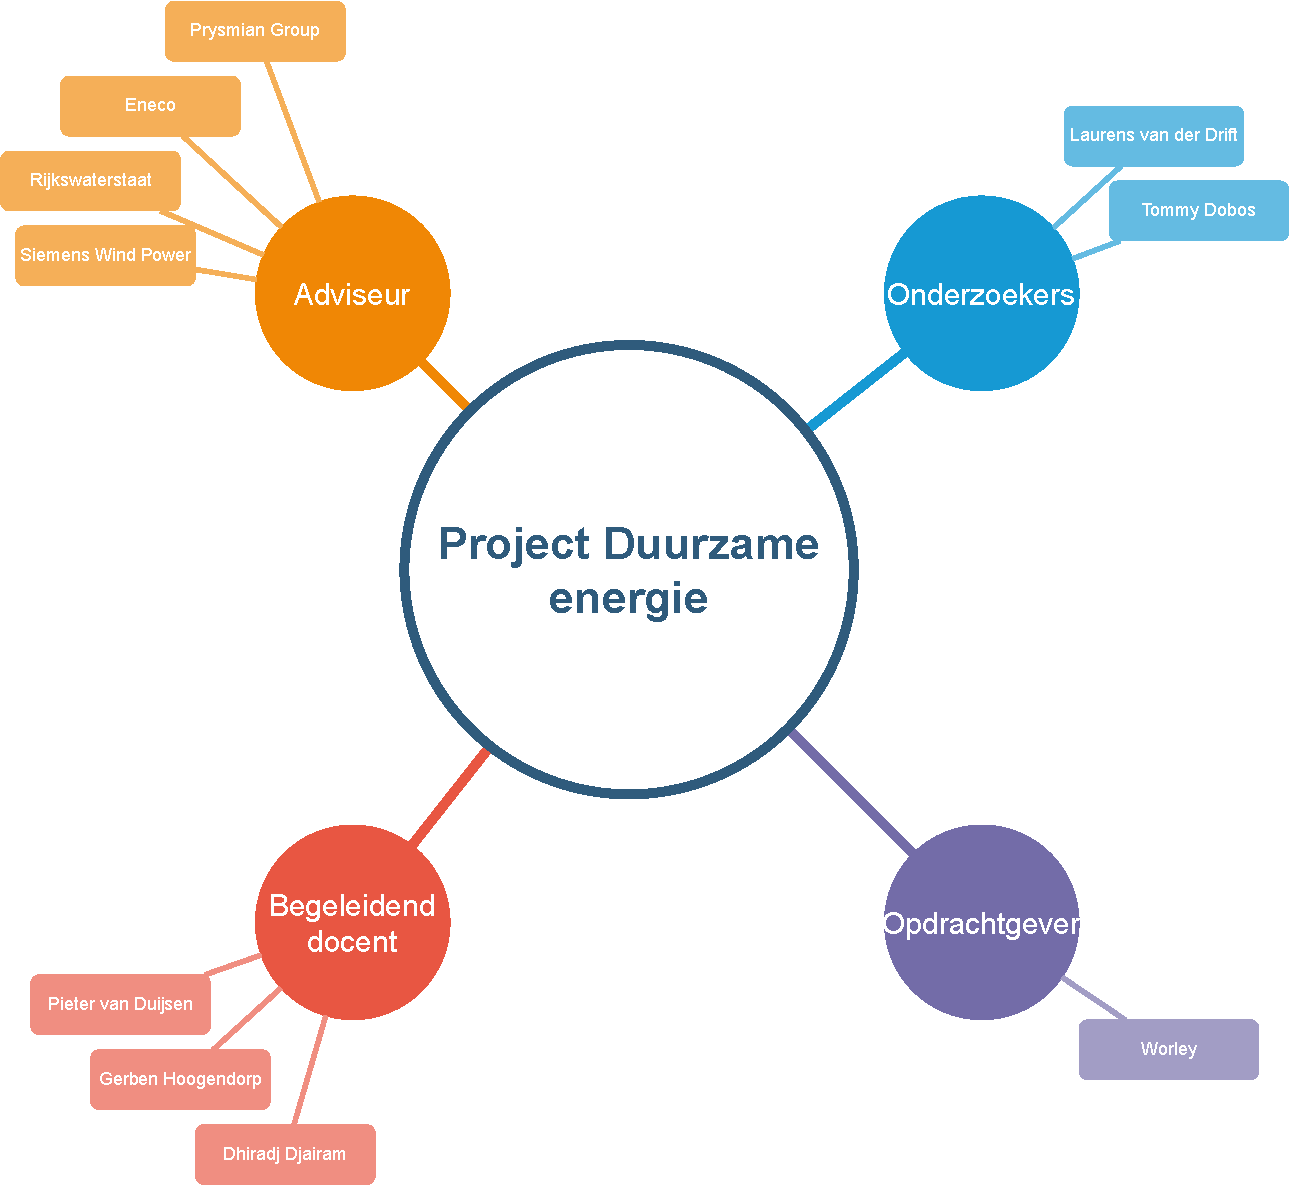
\includepdf[scale=0.65, pages=-]{mindmap/projectorganisatie.pdf}
\end{minipage}
\section{Planning} \label{planning}
We gebruiken de Github planning met drie verschillende weergaven: Overview, ToDoList en roadmap.

In het \textbf{Overview}\textit{(figuur:\ref{fig:overview})} tonen we een samenvatting van alle taken, inclusief degenen die zijn voltooid of nog moeten worden uitgevoerd, met devolgende informatie:

- \textit{Repository}: Aan welk project het onderwerp is gekoppeld\\
- \textit{Titel}: De naam van de opdracht\\
- \textit{Assignees}: Wie verantwoordelijk is voor het uitvoeren van de opdracht\\
- \textit{Status}: De voortgang van de opdracht\\
- \textit{Startdatum} en Deadline: De begin- en einddatum van de opdracht\\
- \textit{Prioriteit}: De urgentie van de opdracht\\

\begin{figure}[h]
    \centering
    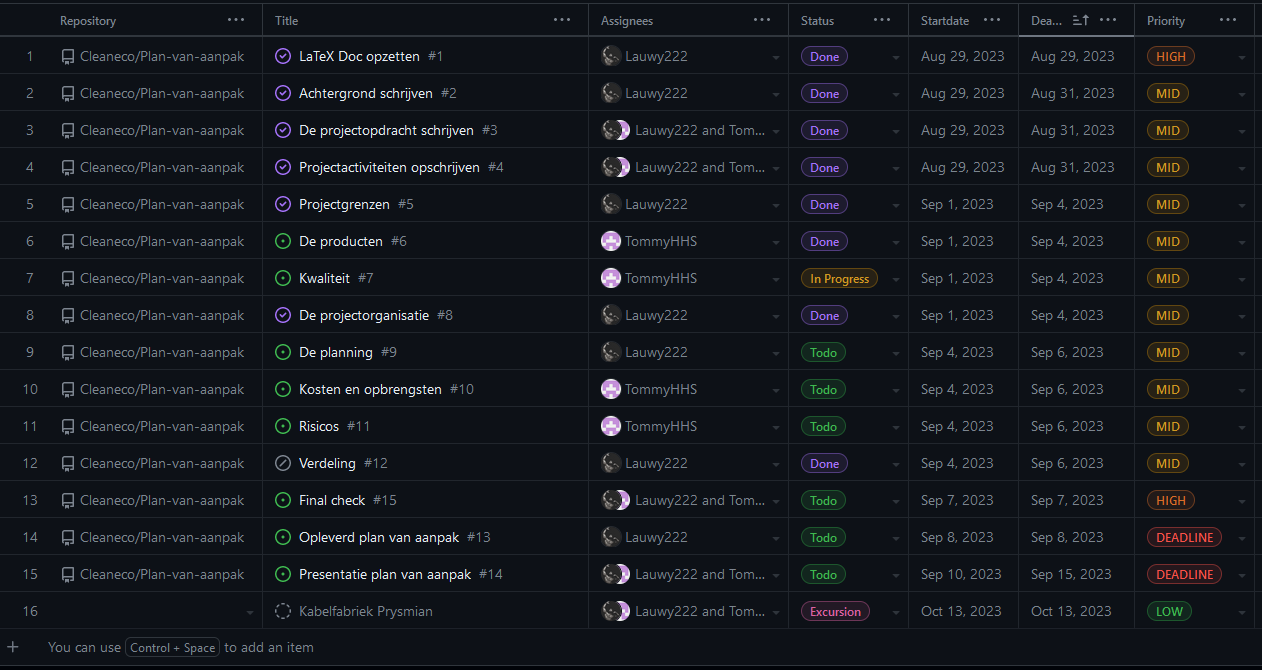
\includegraphics[width=0.9\textwidth]{IMG/overview.PNG}
    \caption{Overview screenshot vanuit GitHub.}
    \label{fig:overview}
\end{figure}

\newpage
In de \textbf{ToDoList}\textit{(figuur:\ref{fig:todolist})} worden vier lijsten weergegeven en gecategoriseerd onder vier koppen: Te doen, In uitvoering, Voltooid en Excursie. Hier geven we aan in welke fase van voltooiing elke opdracht zich bevindt, of het nu nog moet worden gedaan, in uitvoering is, is voltooid, of het een excursie betreft die we moeten voorbereiden.

\begin{figure}[h]
    \centering
    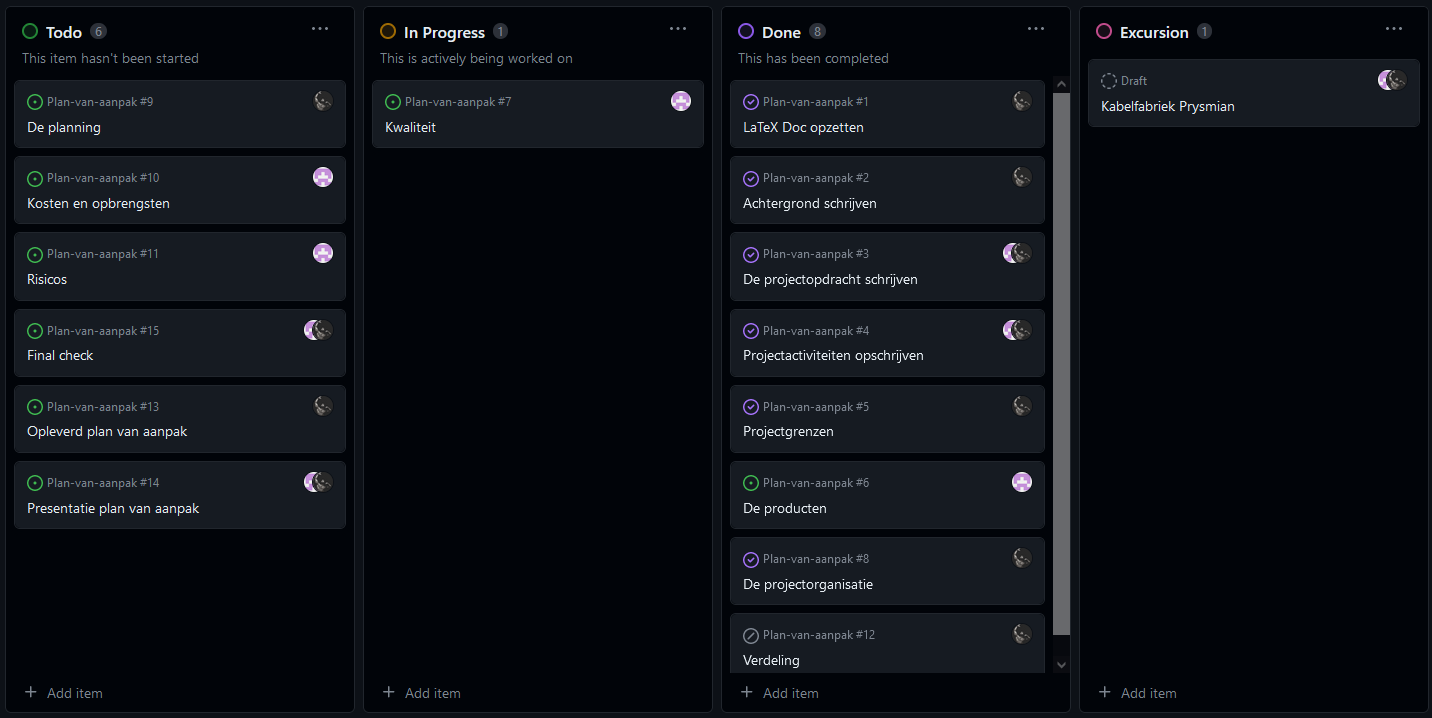
\includegraphics[width=0.9\textwidth]{IMG/todolist.PNG}
    \caption{ToDoList screenshot vanuit GitHub.}
    \label{fig:todolist}
\end{figure}

De \textbf{Roadmap}\textit{(figuur:\ref{fig:roadmap})} toont visueel wanneer een opdracht had moeten beginnen en wanneer de deadline is.

\begin{figure}[h]
    \centering
    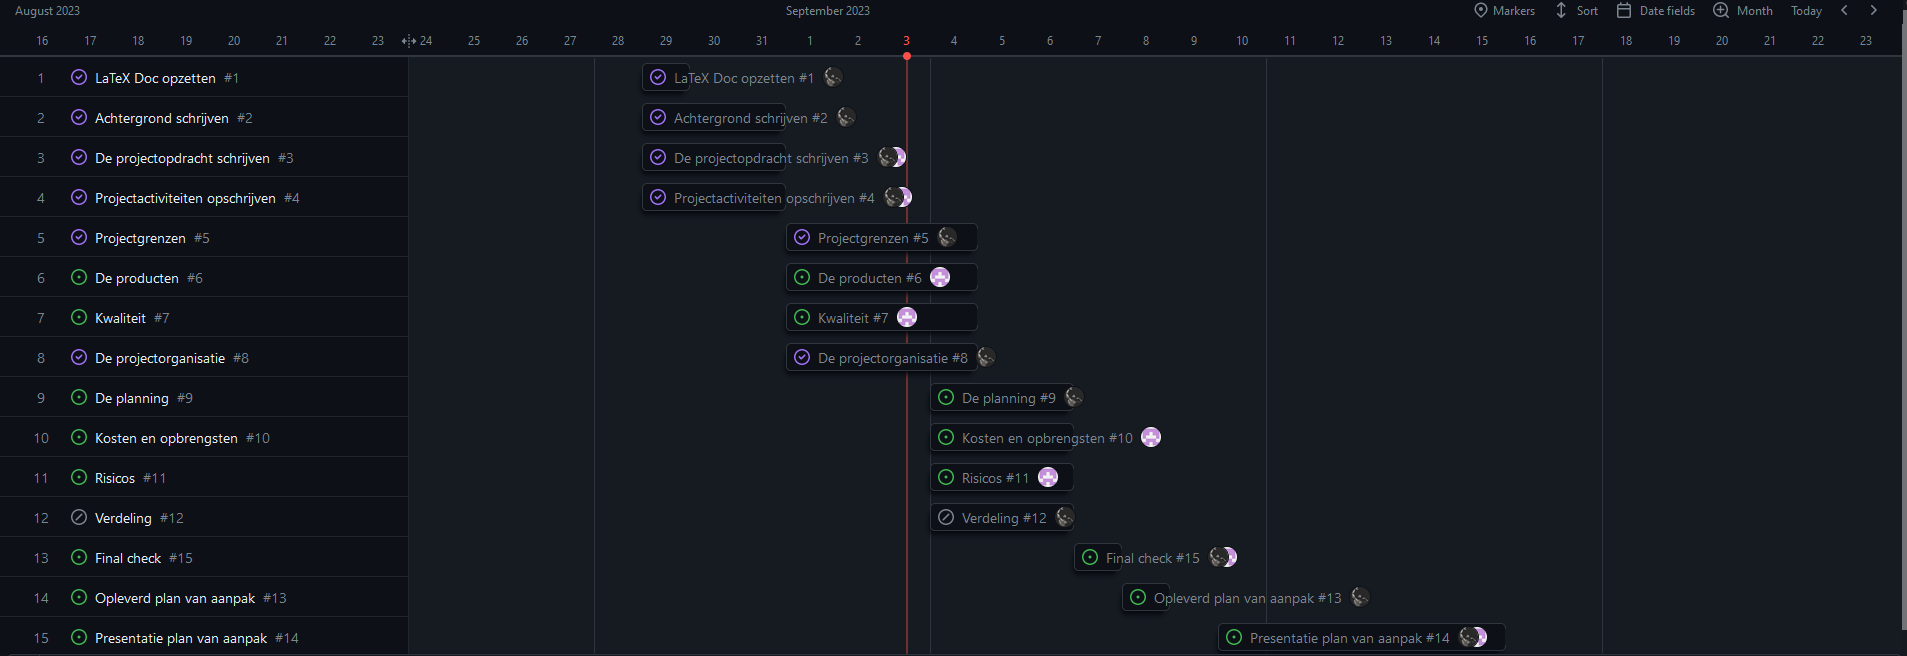
\includegraphics[width=0.9\textwidth]{IMG/roadmap.PNG}
    \caption{Roadmap screenshot vanuit GitHub.}
    \label{fig:roadmap}
\end{figure}
Als er complicaties optreden tijdens het proces van dit project, kunnen we op tijd een opmerking plaatsen en om hulp vragen. Op deze manier zijn we niet beperkt tot fysieke vergaderingen. We kunnen ook per opdracht aangeven wat niet lukt, waardoor alles nog gestructureerder verloopt.



% \section{Planning} \label{planning}
% Wij hebben een planning in Github. Hierin geven wij het volgende aan:

% \textit{- Repository: Aan welk project het onderwerp is gekoppeld}

% \textit{- Title: wat is de titel van de opdracht}

% \textit{- Assignees: wie moet(en) de opdracht maken}

% \textit{- Status: hoe staat het ervoor met de opdracht}

% \textit{- Start-Date en Deadline: wat is de start- en einddatum van de opdracht}

% \textit{- Priority: wat is de urgentie van de opdracht}

% Wij hebben drie verschillende views: Overview, TodoList, Roadmap.

% Bij \textbf{Overview} wordt er een overzicht van alle taken laten zien die al gedaan zijn of nog moeten worden gedaan met extra informatie hierboven genoemd

% Bij \textbf{TodoList} worden er vier lijsten gevisualiseerd geindexeerd door vier kopjes. ToDo, In Progress, Done en Excursion. Hier geven we aan welke opdracht in welke status fase is of dat het een excursie is die wij moeten voorbereiden.

% Bij \textbf{Roadmap} wordt er gevisualiseerd wanneer een opdracht gestart moest zijn en wanneer de deadline is. 


% Mochten er complicaties voorkomen tijdens het process van dit project dan kunnen we optijd een comment plaatsen en vragen om hulp. Zo zijn wij dus niet gelimiteerd aan fysieke meetings. Ook kunnen wij per opdracht aangeven wat er niet lukt en alles dus nog gestructureerder is.


% Elke week worden er opdrachten gemaakt. Bij elke opdracht wordt een begin- en eindtijd gegeven. Het is de bedoeling dat de opdracht binnen deze tijd af is. Zodra dit niet het geval is, zal er eerst in overleg met de groepsleden besproken worden of de eindtijd verschoven mag/kan worden. Als daarentegen de ingeplande tijd voor de betreffende opdracht realistisch was en de opdracht niet af is, zal er in overleg met de opdrachtgever een kort gesprek moeten worden gevoerd om dit in de toekomst te voorkomen. Als er geen verbeteringen te zien zijn in de nabije toekomst, moeten er consequenties worden genomen door de groepsleden en de opdrachtgever.
% Voor de planning wordt Github gebruikt als tool om de opdrachten voor het project duidelijk weer te geven. In figuur 1 is te zien dat één opdracht uit zes kolommen bestaan. Daarin staat de:


% 
\includegraphics[width=6.7in]{IMG/08_planning_01.png} \\
% - Notes: wat moet er worden gedaan om de opdracht te voltooien
% In de opeenvolgende rijen daaronder worden alle opdrachten gemaakt met daarin de bijhorende informatie die in de bovenste kolommen gedefinieerd staan.
% \\\\
\section{Kosten en Opbrengsten}
Het realiseren van zo een project is niet makkelijk en ook niet goedkoop. Daarom zijn de taken gelijkwaardig verdeeld.  In dit hoofdstuk wordt een algemeen overzicht gegeven omtrent de kosten en het tijdschema. Deze organisatie heeft op dit moment vier professionals die dag en nacht in dienst zijn voor dit project. Er moet per groepslid 8 uur per week worden besteed aan het testen van de onderdelen en de gemaakte tussenproducten, het schrijven van de code en alle overige taken voor het project. 

% Please add the following required packages to your document preamble:
% \usepackage[table,xcdraw]{xcolor}
% If you use beamer only pass "xcolor=table" option, i.e. \documentclass[xcolor=table]{beamer}
\begin{table}[h]
\begin{tabular}{|l|l|l|}
\hline
\rowcolor[HTML]{9B9B9B} 
{\color[HTML]{FFFFFF} \textbf{Handeling}} & {\color[HTML]{FFFFFF} \textbf{Beschrijving}} & {\color[HTML]{FFFFFF} \textbf{Aantal}} \\ \hline
\rowcolor[HTML]{EFEFEF} 
Zoekopdracht & \begin{tabular}[c]{@{}l@{}}Met zoekopdrachten wordt verwezen naar de\\ technische problemen die tijdens het proces\\ zijn tegengekomen en die opgelost dienen te\\ worden door een beter systeem te bedenken.\end{tabular} & 8 \\ \hline
Code & \begin{tabular}[c]{@{}l@{}}De structuur van het systeem om het in codes\\ om te zetten\end{tabular} & 8 \\ \hline
\rowcolor[HTML]{EFEFEF} 
Ontwerp & \begin{tabular}[c]{@{}l@{}}Met ontwerp wordt de bruikbaarheid van\\ de auto bedoeld. Dit houd in of de auto compleet,\\ foutloos en storingsvrij functioneert.\end{tabular} & 5 \\ \hline
Raporteren & \begin{tabular}[c]{@{}l@{}}Rapporteren valt onder de documentatie dat\\ gemaakt moet worden tijdens het werken aan\\ het project en onderzoek.\end{tabular} & 2 \\ \hline
\end{tabular}
\end{table}
Gezien de totale handelingen die gedaan dienen te worden om het product te voltooien, zal het in totaal 4 personen 92 uur duren om te creëren. Dit zal 2.760 euro kosten om te voltooien.
\section{Risico’s}
Na het kalibreren, testen en schrijven van de software voor de sensoren en motoren, moet alle software bij elkaar worden gebracht. Het is moeilijk te zeggen hoeveel tijd dit gaat kosten, want het laten werken van de software en het zoeken naar eventuele fouten kan veel tijd in beslag nemen. De deadline voor dit onderdeel is daarom moeilijk te bepalen.

Het verkeerd en niet goed plaatsen van componenten kan onverwachte resultaten geven, waardoor er eventueel meer tijd verloren gaat.
Als tijdens het project een groepslid stopt of door persoonlijke omstandigheden niet door kan gaan met het project, bespreekt de groep hoe dit wordt opgelost. In dit geval zal elk groepslid per week meer tijd moeten besteden aan het project.

Bij gebrek aan kennis, wordt verwacht dat er eerst goed onderzoek wordt gedaan en de benodigde kennis wordt opgedaan. Als het niet lukt om de benodigde informatie te vinden, zal er naar alternatieve externen moeten worden gekeken.
Als tijdens het project extra budget nodig is voor defecte sensoren en motoren, moet in overleg met de opdrachtgever naar een oplossing worden gezocht. Bij het gebrek aan budget door defecte sensoren, motoren of andere componenten, wordt in overleg met de opdrachtgever gekeken of dit kan worden opgelost.

% \section{Verdeling van hoofdstukken}
 % Please add the following required packages to your document preamble:
% \usepackage[table,xcdraw]{xcolor}
% If you use beamer only pass "xcolor=table" option, i.e. \documentclass[xcolor=table]{beamer}
\begin{table}[h]
\begin{tabular}{|r|l|}
\hline
\rowcolor[HTML]{9B9B9B} 
\multicolumn{1}{|c|}{\cellcolor[HTML]{9B9B9B}\textit{\textbf{Hoofdstuk}}} & \multicolumn{1}{c|}{\cellcolor[HTML]{9B9B9B}\textit{\textbf{Teamlid}}} \\ \hline
\rowcolor[HTML]{EFEFEF} 
1 & Francisco Ramirez Ramirez \\ \hline
2 & Laurens van der Drift \\ \hline
\rowcolor[HTML]{EFEFEF} 
3 & Tommy Dobos \\ \hline
4 & Justin van der Reijden \\ \hline
\rowcolor[HTML]{EFEFEF} 
5 & Laurens van der Drift \\ \hline
6 & Tommy Dobos \\ \hline
\rowcolor[HTML]{EFEFEF} 
7 & Francisco Ramirez Ramirez \\ \hline
8 & Justin van der Reijden \\ \hline
\rowcolor[HTML]{EFEFEF} 
9 & Francisco Ramirez Ramirez \\ \hline
10 & Justin van der Reijden \\ \hline
\rowcolor [HTML]{EFEFEF}
Eindredactie & Tommy Dobos \\ \hline
\end{tabular}
\end{table}
\phantomsection
\addcontentsline{toc}{section}{Referenties}
\printbibliography
\end{document}
